\hspace{24pt}
% \renewcommand{\baselinestretch}{1.5}

\section{Background}
The bodies of humans and other complex animals are composed of trillions of cells.  Those cells can be classified into a large number (hundreds at least) of cell types which look and behavior radically different from each other (e.g.\ information processing neurons, insulin secreting $\beta$-cells, protective skin cells, etc.).  These cells are specialized to do particular tasks and the retain their identify during cell division; for example when a skin cell divides the outcome is two skin cells.  Interestingly, the basic nucleotide sequence of the genomes of these diverse cell types is essentially the same.  How then can these cell types be distinct?  The answer is thought to largely lie in differences in so called ``epigenetic marks'', namely DNA methylation and various histone modifications.

\subsection{DNA Methylation}
DNA methylation refers to the covalent addition of a methyl group to DNA nucleotides.
In vertebrates the primary form of DNA methylation is the addition of a methyl group to the C5 carbon residue of cytosines (fig.~\ref{f2}).  The reaction is catalyzed by DNA methyltransferases which act on cytosines found in CpG dinucleotides.  Some DNA methyltranferases function to maintain the methylation state of CpG's during cell division, ensuring that both daughter cells end up with methylated cytosines in the same places.  DNA methylation is heavily studied for two reasons.  First, DNA methylation can be measured more precisely and accurately than other epigenetic marks (via bisulfite sequence~\cite{frommer1992bisulfite}) and it is highly stable (DNA methylation is still largely intact after storage at 4$^{\circ}$C for 20 years ~\cite{li2018stability}).  Second, DNA methylation is known to be involved in several key biological processes, including regulation of gene expression, cell differentiation, and so on \cite{krueger2012dna}.

\begin{figure}[ht]
    \centering
    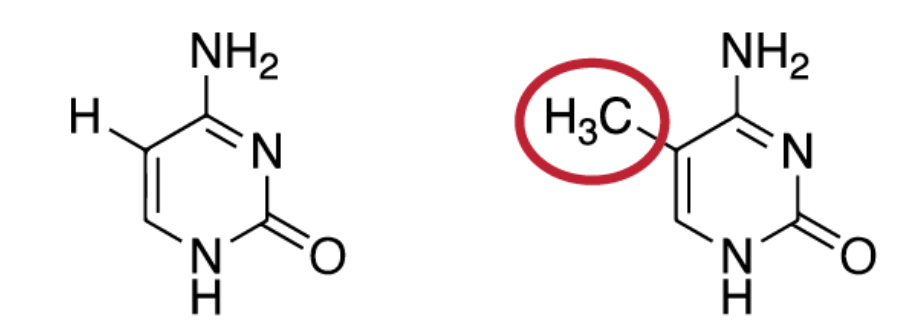
\includegraphics[width=0.8\columnwidth]{body/figure/figure2.png}
    \captionsetup{labelfont=bf}
    \renewcommand{\baselinestretch}{1.0}
    \caption[An illustration of DNA methylation]{The chemical structure of methylated (right) and unmethylated cytosine (left) is shown. (figure reproduced from \cite{enwiki:1028802025})}
    \label{f2}
\end{figure}


\subsection{Histone Modification}
Histones are a kind of structural DNA-binding protein that pack and order the DNA of eukaryotic chromosomes into basic structural units, called nucleosomes. A nucleosome consists of a segment of DNA, roughly 147 base pairs, wound around eight histone proteins. These are two copies of the four core histones (H2A, H2B, H3, H4) which form the structure, known as a histone octamer. Meanwhile, the H1 histone acts as the linker histone to stabilize inter-nucleosomal DNA but is not a one of core histones in the octamer.

\begin{figure}[H]
    \centering
    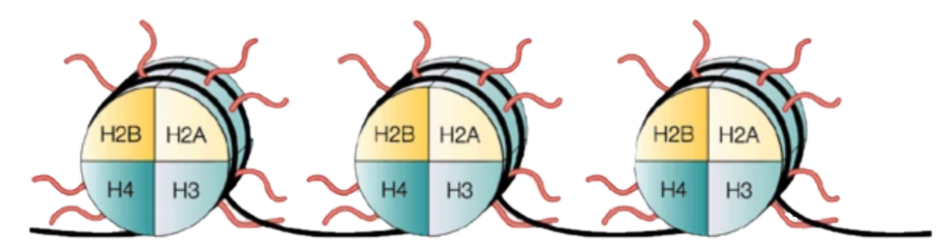
\includegraphics[width=1\columnwidth]{body/figure/figure1.png}
    \captionsetup{labelfont=bf}
    \renewcommand{\baselinestretch}{1.0}
    \caption[Structure of nucleosome]{The black curve is double-stranded DNA chain. It wraps around the eight core histones, and composes a spherical structure called a nucleosome. The red line is amino N-terminal tail, is major the part of occurring modification. (figure from \cite{marks2001histone})}
    \label{f1}
\end{figure}

Histone modification refers to covalent post-translational modification to histone amino N-terminal tail, including methylation, acetylation, phosphorylation and so on. Among these, the most common modifications are the methylation of arginine or lysine, and the acetylation of lysine. Histone modification affects a variety of biological processes, such as transcriptional activation and inactivation \cite{luger1997crystal}, as well as chromosome packaging \cite{peterson2004histones}, by altering structure \cite{allfrey1964acetylation} or recruiting histone modifier. Additionally, histone modifications are also helpful to identify some gene-regulatory regions. In Table\ref{t1}, it shows the five core histone marks and one histone acetylation mark, proposed by Roadmap Epigenomics Consortium \cite{kundaje2015integrative}, that are highly associated with different regulatory regions. According to these literatures, histone modifications play vital role in epigenetic research and provide useful information for further analysis.

\begin{table}[H]
    \centering
    \begin{tabular}{lc}
        \hline
        Histone modification    & Regulatory region \\\hline
        H3 lysine 4 monomethylation (H3K4me1) & Enhancer regions \\
        H3 lysine 4 trimethylation (H3K4me3)   & Promoter regions \\
        H3 lysine 9 trimethylation (H3K9me3) & Heterochromatin regions \\
        H3 lysine 27 acetylation (H3K27ac) & Enhancer regions \\
        H3 lysine 27 trimethylation (H3K27me3) & Polycomb repression \\
        H3 lysine 36 trimethylation (H3K36me3) & Transcribed regions \\\hline
    \end{tabular}
    \captionsetup{labelfont=bf}
    \caption{Table of histone modifications corresponding to regulatory regions}
    \label{t1}
\end{table}


\section{Problem Description}
In order to better understanding of epigenetic mechanism, quantitative detection of histone modification is important. Histone modifications are mainly profiled by chromatin-immunoprecipitation followed by sequencing (ChIP-seq). This method uses corresponding antibody for histone modifications or specific DNA-binding proteins to identify enriched loci within genome \cite{nakato2020methods}. The major advantage of ChIP-seq is the higher resolution and lower noise over chromatin immunoprecipitation with DNA microarray (ChIP-chip) \cite{massie2012mapping}. But, the disadvantage of ChIP-seq is still expensive and time-consuming, because it requires lots of tissues, so that profiling rare biological samples, such as primary cells and clinical samples, is constrained \cite{gilfillan2012limitations}. In this case, these biosamples may be rejected low-quality data resulting in the missing value, or identified lower quality data. It will cause bias in further analysis. Thus, data imputation methods are often used appropriately in this scenario.

Data imputation with computational methods attempt to utilize relation among different kinds of biological data to remove noise or reconstruct missing value. Currently, multiple public datasets are available to download. They are provided by the project conducted international collaboration of research groups, such as Encyclopedia of DNA Elements (ENCODE) project \cite{davis2018encyclopedia} and Roadmap Epigenomics project \cite{kundaje2015integrative}. These lots of available data is good for data imputation with computational method. Especially, machine-learning based or deep-learning based methods are data-driven approaches that are good at dealing with large amount of data. Thus, diverse bioinformatics studies in recent massively apply deep-learning methods, and expect a variety of frameworks of deep learning to discovery more insight in biological domain.

The most popular frameworks, convolutional neural network (CNN) and recurrent neural network (RNN), are extensively used to extract features. These are individually great at modeling translation invariant features by CNN, and modeling long-range interactions by RNN. According the properties of frameworks and biological data, we can choose the most appropriate model to fit on diverse tasks. For example, DeepBind uses CNN to predict binding site of DNA and RNA binding proteins by extracting features from DNA sequences, and allows to learn the correct motifs by different kernels in CNN \cite{alipanahi2015predicting}. Quang and Xue proposed new hybrid framework, called DanQ, that combines CNN and bi-directional long-short term memory(BiLSTM) network, which is a variant of RNN. It takes advantages of these frameworks to predict the functions of DNA sequences \cite{quang2016danq}. Min et al. proposed a deep learning framework, called DeepEnhancer, to classify enhancer regions from genomic sequences \cite{min2016deepenhancer}. The success of these methods shows that deep learning is a powerful tool for genomic researches. However, DNA sequences in different cell lines are identical. Above successful methods only extract features from DNA sequences, so that these methods are lack of power of making predictions in cell line-specific cases \cite{yin2019deephistone}\cite{chen2021deepcape}.

\section{Motivation}
Therefore, to overcome this limitation, there are many deep-learning based methods integrating DNA sequences and various biological experimental data. For example, Laiyi Fu et al. proposed a hybrid deep learning model additionally adding features from MeDIP-seq data and information of histone modification to predict DNA methylated states \cite{fu2019predicting}. Chen et al. proposed DeepCAPE, a deep CNN to predict enhancers via the combination of DNA sequences and DNase-seq data \cite{chen2021deepcape}. These papers in cell line-specific manner improve performance of data imputation for epigenetic data.

Besides, DNA methylation and histone modification not only individually supply useful insight in analysis but also have special interaction between themselves. Recent evidence indicates that DNA methylation and histone modification pathways can be interdependent, and this crosstalk can be mediated by biochemical interaction. For example, histone modification can directly help to DNA methylation, and DNA methylation might serve as a template for some histone modifications \cite{cedar2009linking}. As such, it is rational to integrate DNA sequences and DNA methylation information for the study of cell line-specific histone modifications.

\section{Objective}
In our research, we aim to find out whether introducing information from DNA methylation can help to improve prediction of binding sites of histone modifications. Motivated by the above understanding, we design deep-learning based approach to capture features from DNA sequences, while taking advantage of the relationship between histone modifications and DNA methylation signal. In order to ensure whether our hypothesis is effective, we use comprehensive experiments to validate our approach.
